% !TEX root = MMMK.tex

\section{Overview}

\begin{figure}[ht]
\centering
\includegraphics[width=10cm]{images/OverviewYoung.png}
\caption{Overview according to Young}
\label{fig:overviewYoung}
\end{figure}

\begin{figure}[ht]
\centering
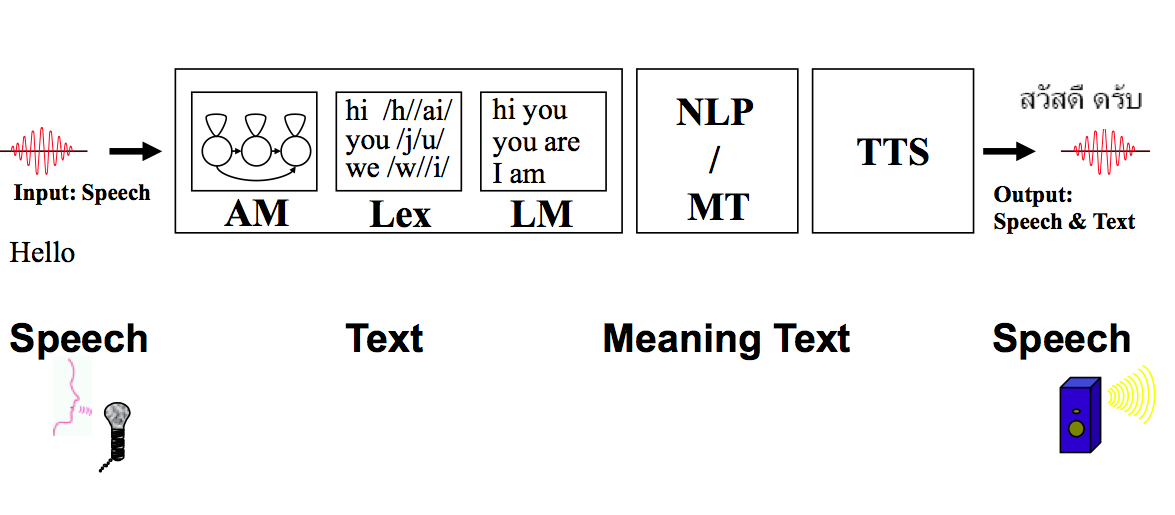
\includegraphics[width=10cm]{images/OverviewSchultz.png}
\caption{Overview according to Schultz}
\label{fig:overviewSchultz}
\end{figure}

\newpage

\section{Introduction}

\subsection{Why do we need Automatic Speech Recognition (ASR)?}

\begin{center}
  \begin{tabular}{ c | c }
    \hline
    Advantages & Disadvantages  \\ \hline
    Speech is a natural way of communication & When you are not allowed to speak, it is unusable   \\
    Allows an additional communication channel   & Unsatisfactory recognition rate  \\
    Hands and eyes are free for other tasks & Problems with accents, dialects and code-switching   \\
    Mobility & Cultural factors (e.g. uncertainty avoidance)   \\
    Some communication channels are speech-only & Speech input is still more expensive   \\
    \hline
  \end{tabular}
\end{center}

\begin{figure}[ht]
\centering
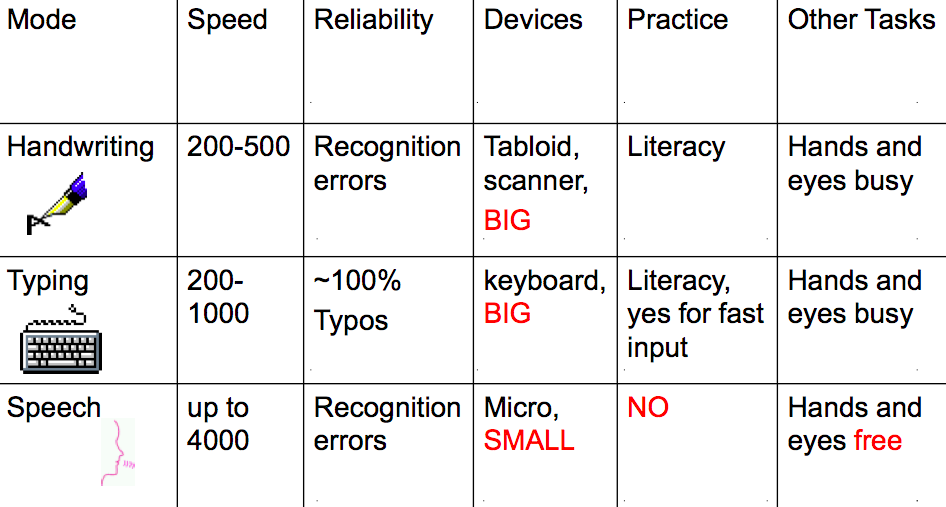
\includegraphics[width=10cm]{images/Input.png}
\caption{Input Characters per minute}
\label{fig:inputCharacters}
\end{figure}

\subsection{Where is Speech Recognition and Understanding useful?}
\subsubsection{Human-Machine Interaction}
\begin{enumerate}
\item Applications for Remote Control
\begin{itemize}
\item Using the phone to operate machines
\end{itemize}

\item Hands/eyes are busy or not usable
\begin{itemize}
\item Speech recognition while driving
\item Nurse bots for physically disabled
\end{itemize}

\item Authentication
\begin{itemize}
\item Speaker Identification/Verification/Segmentation
\item Language/Accent Identification
\end{itemize}

\item Entertainment

\item Indexing and Transcribing Acoustic Documents
\begin{itemize}
\item Archive, Summarize, Search and Data Retrieval
\end{itemize}

\end{enumerate}

\subsubsection{Human-Human Interaction}
\begin{enumerate}
\item Communication across language barriers
\begin{itemize}
\item Simultaniously translating one language into the other
\end{itemize}

\item Support human interaction
\begin{itemize}
\item Meeting and lecture systems
\item Speech therapy support

\end{itemize}


\end{enumerate}



\section{Basics}

\subsection{Why is ASR so difficult?}
\begin{itemize}
\item Complexity
\begin{itemize}
\item typically 32000 Bytes per second (\textbf{amount of data})
\item 50 phonemes, 5000 sounds, 100000 words (\textbf{class inventory})
\item exponential growth of possible sentences (\textbf{combinatorial explosion})
\end{itemize}

\item Segmentation
\begin{itemize}
\item no boundary markers 
\item continous flow of samples
\end{itemize}

\item Variability
\begin{itemize}
\item anatomy of vocal tract, speed, loudness, stess, dialect, mood (\textbf{speaker})
\item noise, channel conditions, cocktail effect (\textbf{channel, enviroment})
\end{itemize}

\item Ambiguity
\begin{itemize}
\item similar sounding words (\textbf{homophones})
\item interface vs in her face (\textbf{word boundaries})
\item He saw the Grand Canyon flying to New York (\textbf{semantics})
\item Time flies like an arrow (\textbf{practmatics})

\end{itemize}


\end{itemize}


\subsection{Speech units}

\begin{itemize}
    \item \textbf{phone}: a sound one produces, such as [p]
    \item \textbf{phoneme}: an abstract unit, such as /h/
    \item \textbf{morpheme}: the smallest part of speech with semantic meaning, for example un-break-able
\end{itemize}

When the meaning of an utterance can be changed by replacing one phone in the utterance with another phone, the replaced phone and the phone that replaces it are said to form a \textbf{minimal pair}.
A phoneme may correspond to one phone or a set of phones. In the latter case, all phones of the set are called \textbf{allophones} of the phoneme.
For example, /o/ and /u/ are phonemes in English because there are minimal pairs that differ only in these phonemes, such as ''bone`` and ''boon``. The English phoneme /p/ has two allophones, one with aspiration and one without it.

\subsection{Problems with different Languages}
More detailed LM-Handeling in chapter 7.9!
\begin{itemize}
\item{Words:}
\begin{itemize}
\item{Indo-European:} Segmentation via whitespace
\item{Japanese, Chinese, Thai:} No segmentation
\end{itemize}

\item{Spoken words:} Words are not marked by boundaries. Units can have intonation phrases (like , )

\item{Compunding (e.g. German):} Donau-Schiff-Fahrts-Kapitäns-Mütze 
\begin{itemize}
\item \emph{How to handle}: Decompose compound words into constituent parts and carry out pronounciation and language modelling on the decomposed parts
\end{itemize}
 
 \item Highly inflected languages(e.g. Turkish, Arabic, Slavic): \emph{Inflection:} Modification of a word to express different grammatically categories (e.g. David-san) 
 \begin{itemize}
 \item \emph{How to handle:} Specific components for modelling inflection (like morpheme based modelling)
 \end{itemize}

\end{itemize}


\subsection{$k$-means clustering}

Given an observation $(x_1, \ldots, x_n)$, find $k \leq n$ clusters $S = \left\{S_1, \ldots, S_k\right\}$, such that:

\[
    \argmin_S \sum\limits_{i = 1}^k \sum\limits_{x_j \in S_i} ||x_j - \mu_i||^2
\]

where $\mu_i$ is the mean of points in $S_i$.

\subsection{Comparing two utterances}

Major problems:
\begin{itemize}
\item When does the utterance start?
\item \emph{Solution: Speaker has to push/ Always records and pattern recognition}
\item Number of speech vectors is varying (speaker-dependent, on purpose, non purposely)


\item \emph{Solution:} Dynamic Time Warping

    \begin{itemize}
    \item works like the dynamic editing distance algorithm (DP)
    \item Cost function: vector-vector distance
    \item \emph{Pro:} 
    \begin{itemize}
    \item only needs current and previous frame 
    \item solves the different time-axis-alignment problem
    \end{itemize}
    
    \item{\emph{Cons:}}
    \begin{itemize}
    \item Does not generalize
    \item Speaker dependent
    \item Need examples for each word for each speaker
    \item Computationally expensive for large vocabularies
    \item Continous speech cannot be segmentated except for human recognition because of \textbf{Co-Articulation, Hesitation and Hard decisions}.
    \item $\rightarrow$ Works only for small vocabularies, speaker dependent recognition and isolated words
    \end{itemize}

\end{itemize}

    \end{itemize}

\newpage

\section{Signal processing}
Remember: Parametric representation depends on targeted application (speech coding, speech synthesis, speech recognition)
\subsection{How can we extract features?}

Our goal: Continous signal $\rightarrow$ Discrete representation

\begin{itemize}
\item sampling (x-Axis)
\begin{itemize}
\item Aliasing possible if sampling rate is not at least 2 times maximal frequency (Nyquist or sampling theorem)
\end{itemize}

\item quantization (y-Axis)
\begin{itemize}
\item SNR (Signal to Noise Ratio) $\frac{power\left(signal\left[i\right]\right)}{power\left(noise\left[i\right]\right)}$
\item SNR low $\rightarrow$ Recognition performance is low
\item speech signal is usually between 50dB and 60dB
\end{itemize}

\end{itemize}

\subsection{Acoustic Features in sampled signal}
\begin{itemize}
\item Amplitude
\item Power (Integral of squared signal)
\begin{itemize}
\item useful for detecting speech, syllabus, phrase boundaries
\end{itemize}
\item Peak to Peak
\item Root mean square
\item Zero crossing
\begin{itemize}
\item can help distinguishing some weak sounds from silence
\end{itemize}
\item voiced/unvoiced


\end{itemize}

\subsection{Frequency domain and Fouriertransformation}
Why preform signal processing in the frequency domain?
\begin{itemize}
\item Human hearing is based on frequency analysis
\item Use of frequency analysis often facilitates understanding
\item Use of frequency analysis often simplifies signal processing
\end{itemize}

We can transform signals from time domain into frequency domain via \textbf{Fouriertransformation} 
\begin{itemize}
\item \emph{continuous}: $F\left(w\right) = \int f\left(t\right)e^{-iwt}dt$ - inverse: $f\left(t\right) = \frac{1}{2\pi}\int F\left(w\right)e^{-iwt}dw$ 
\item \emph{discrete}: $F\left(x\left[k\right]\right) = \sum x\left[k\right]e^{-iwt}dt$ - inverse: $x\left[k\right] = \frac{1}{2\pi}\int F\left(x\left[k\right]\right)e^{-iwt}dw$ 
\end{itemize}
Fouriertransformation have got some useful computational properties:
\begin{itemize}
\item Modelling a channel often can be accomplished by \emph{convolution}
\item A \emph{convolution} in time domain is a \emph{multiplication} in frequency domain and a \emph{summation} in log-frequency domain
\item Due to invertibility no information is lost
\end{itemize}


\subsection{Short-Term Spectral Analysis}

Problem: Frequency over an entire utterance does not help much because most acoustic events are not static, have durations in the range of 10 to 100ms and need more detailed analysis.  \\

Idea: To better analyse our utterance we partition the utterance into short segments which may overlap each other. This is done by short-term spectral analysis. \\

The general idea of short-term spectral analysis is to

\begin{itemize}
    \item multiply the speech signal with a window function
    \begin{itemize}
    \item \emph{Reason:} Conventional fourier analysis does not capture time varying nature. \\ Furthermore it smooths the resulting spectrum
    \item \emph{Some popular window functions:} Hamming (most used), Hanning, Rectangle, Gaussian
    \end{itemize}

    \item apply the Discrete Time Fourier Transform (DTFT)
    \item use a filterbank (such as \textit{Mel} or \textit{Bark})
    \begin{itemize}
    \item \emph{Reason:} Fourier coefficients reflects too much of the signals microstructure which contains a lot of redundancies and misleading information. We have to filter according to the human ear (works also with filterbanks!)
    \end{itemize}

\end{itemize}

\emph{Notice:} Instead of multiplying the speech signal with a window function and applying DTFT afterwards, you can also apply DTFT on the window function first and then multiply with the speech signal. The result will be the same.
\subsection{Linear Predictive Coding}

LPC is an alternative to Fourier analysis. When using LPC, we assume that a speech signal is produced by a buzzer (\textit{glottis}) at the end of a tube (\textit{vocal tract}), with occasional added hissing and popping sounds. Then, the intensity and frequency can be estimated with linear prediction:

\begin{equation}
    \tilde{s}(n) = \sum\limits_{i = 1}^p \alpha_i s(n - i)
\end{equation}

Some sounds, for example nasal sounds, cannot be described by this model. This means that there will be an error, called the residue, which is stored and used to model other sounds:

\begin{equation}
    e(n) = s(n) - \tilde{s}(n)
\end{equation}

The goal of the prediction is to minimize the squared error $\sum e(n)^2$. This error can be further transformed into cepstral coefficients using the Z-transform.

\subsection{Cepstra}

The speech signal $s(n)$ can be described by a convolution of stimulating signal $u(n)$ (caused by the glottis) and an impulse response $h(n)$ (caused by the vocal tract and the lips):

\begin{equation}
    s(n) = u(n) \ast h(n)
\end{equation}

In speech analysis, we are particularly interested in discovering the formant structure. This means that we have to ''get rid`` of the stimulating signal:

\begin{equation}
    \mathcal{F}(s) = \mathcal{F}(u) \cdot \mathcal{F}(h)
\end{equation}

\begin{equation}
    \mathcal{F}^{-1}(\log(\mathcal{F}(s))) = \mathcal{F}^{-1}(\log(\mathcal{F}(u))) + \mathcal{F}^{-1}(\log(\mathcal{F}(h)))
\end{equation}

Note that after the inverse Fourier transform, we are not in the time domain, but in the cepstral domain (also called quefrency). The lower cepstral coefficients describe the macro structure of the signal whereas the higher cepstral coefficients describe the micro structure of the signal. Thus, the higher cepstral coefficients are often discarded.

In order to separate the signal's components, we have to apply a \textit{lifter} (setting some of the coefficients to 0) to filter out the information we need. This is done by removing cepstral summits with a lowpass lifter.

A cepstrum in general is:
\begin{itemize}
\item efficient and robust coding of speech information
\item information about rate of change in the different spectrum bands
\item useful for seperating signals (like the source and filter in the Source-Filter-Model)
\end{itemize}


\subsubsection{Mel-frequency cepstrum (MFC)}

MFCCs are coefficients that collectively make up an MFC. 
MFCCs are commonly derived as follows:

\begin{enumerate}
    \item segment incoming waveforms into frames (10ms)
    \item apply the Fourier transform to a signal to compute frequency response
    \item group the frequency response into 25-40 buckets by applying a Mel filterbank (triangular weighting function)
    \item take the $\log$ of the powers at each Mel ''bucket``
    \item take the discrete cosine transform (DCT) of the list of mel log powers
    \item the MFCCs are the amplitudes of the resulting spectrum
\end{enumerate}

Usually, we take the first coefficient (the power of the signal) and 12 more coefficients, amounting to a total of 13 numbers.

\subsection{Feature vectors}

During further processing, we often assume that the speech signal at a given point of time is independent from the signal before and after that point of time. This is a poor assumption. So, if we have a feature vector $x$ (if we're using MFCCs, we have 13 coefficients), we also store the first and second derivatives of $x$, namely $\Delta x$ and $\Delta \Delta x$ (if we're using MFCCs, we now have 39 numbers - a huge reduction, compared to 8000 numbers in the original speech signal).

\newpage

\section{Hidden Markov Models}

\subsection{Why do we use HMMs?}
\begin{itemize}
\item mathematical foundation
\item works with speech units shorter than words
\begin{itemize}
\item subword unit occurs often
\item training easier
\item less data required
\end{itemize}
\item Recognize speech from any speaker
\item Recognize continous speech
\item Recognize untrained words due to subwords compositions

\end{itemize}


\subsection{The three great problems}

\subsubsection{Evaluation}

\textbf{Problem:} Given an HMM $\lambda$ and an observation $O = (x_1, \ldots, x_T)$, compute the probability $P(x_1, \ldots, x_T | \lambda)$.

\vspace{10pt}

\textbf{A weaker problem:} Given an HMM $\lambda$ an observation $O = (x_1, \ldots, x_T)$ and a state sequence $(s_{q_i}, \ldots, s_{q_T})$, compute the probability $P(x_1, \ldots, x_T | \lambda, (s_{q_1}, \ldots, s_{q_T}))$.

\vspace{5pt}

\textbf{Solution:}
\begin{equation}
    \pi(s_{q_1}) b_{q_1}(x_1) \prod\limits_{k = 1}^{T - 1} a_{q_{k}q_{k+1}} b_{q_{k+1}}(x_{k+1})
\end{equation}
This solution is of course not applicable to the evaluation problem because the state sequence is unknown.

\vspace{10pt}

\textbf{Solution: the Forward algorithm}. Define:

\begin{equation}
    \alpha_1(j) = \pi(s_j) \cdot b_j(x_1)
\end{equation}

\begin{equation}
    \alpha_t(j) = \sum\limits_i a_{ij} \cdot \alpha_{t-1}(i)
\end{equation}

\subsubsection{Decoding}

\textbf{Problem:} Given an HMM $\lambda$, and an observation $O = (x_1, \ldots, x_T)$, find the most likely state sequence $s_{q_1}, \ldots, s_{q_T}$:

\begin{eqnarray*}
    \argmax_{(q_1, \ldots, q_T)} P(q_1, \ldots, q_T \bigm| x_1, \ldots, x_T, \lambda)
    &=& \argmax_{(q_1, \ldots, q_T)} \frac{P(q_1, \ldots, q_T, x_1, \ldots, x_T \bigm| \lambda)}{P(x_1, \ldots, x_T \bigm| \lambda)} \\
    &=& \argmax_{(q_1, \ldots, q_T)} P(q_1, \ldots, q_T, x_1, \ldots, x_T \bigm| \lambda)
\end{eqnarray*}

\textbf{Solution: the Viterbi algorithm}. Define:

\begin{equation}
    z_1(j) = \pi(j) \cdot b_j(x_1)
\end{equation}

\begin{equation}
    z_t(j) = \max_i(a_{ij} \cdot z_{t-1}(i)) \cdot b_j(x_t)
\end{equation}

Both the Forward and the Viterbi algorithm often multiply many small numbers. This can lead to floating point underflow errors. As a solution, one can either scale the factor by a constant or use logarithms to turn the multiplications into additions.

\subsubsection{The Backward algorithm}

Obviously:

\begin{equation}
    P(x_1, \ldots, x_T \bigm| \lambda) = \sum\limits_i P(x_1, \ldots, x_T, q_t = i \bigm| \lambda)
\end{equation}

Define:

\begin{equation}
    \beta_t(i) = P(x_{t+1}, \ldots, x_T, q_t = i \bigm| \lambda)
\end{equation}

\vspace{10pt}

$\beta_t(i)$ is the probability of observing the partial observation $x_{t+1}, \ldots, x_T$ and being in state $s_i$. Then:

\begin{enumerate}
    \item Initialization: $\beta_T(i) = N^{-1}$
    \item Induction: $\beta_t(i) = \sum\limits_j a_{ij} \cdot b_j(x_{t+1}) \cdot \beta_{t+1}(j)$
    \item Termination: $P(x_1, \ldots, x_T \bigm| \lambda) = \sum\limits_j \beta_T(j)$ (shouldn't this be $\sum\limits_j \beta_1(j)$?)
\end{enumerate}

\subsubsection{Learning / optimization}

\textbf{Goal:} Given an observation $O$ and an HMM $\lambda$, find another HMM $\lambda'$ such that $P(O \bigm| \lambda') > P(O \bigm| \lambda)$.

\textbf{Solution:} We use the Baum-Welch algorithm, which is an EM algorithm (expectation-maximization). The Baum-Welch algorithm uses a forward-backward procedure.

First, define $\gamma_t(j)$, which is the probability that the system $\lambda$ is in state $s_j$ at time $t$ when producing the observation $X = (x_1, \ldots, x_T)$:

\begin{equation}
    \gamma_t(j) = \frac{P(q_t = j \bigm| X, \lambda)}{P(X \bigm| \lambda)} = \frac{\alpha_t(j) \cdot \beta_t(j)}{\sum\limits_i \alpha_t(i) \cdot \beta_t(i)}
\end{equation}

To optimize $a_{ij}$, we need the probability $\xi_t(i, j)$ of being in state $i$ at time $t$, transition from state $i$ to $j$ and be in state $j$ at time $t+1$.

\begin{eqnarray*}
    P(q_t = 1, q_{t+1} = j \bigm| X, \lambda) &=& \frac{P(q_t = 1, q_{t+1} = j, X \bigm| \lambda)}{P(X \bigm| \lambda)} \\
                                              &=& \frac{\alpha_t(i) \cdot a_{ij} \cdot b_j(x_{t+1}) \cdot \beta_{t+1}(j)}{P(X \bigm| \lambda)} \\
                                              &=& \xi_t(i, j)
\end{eqnarray*}

As a reminder (this follows from the rules of conditional probabilities):

\begin{equation}
    P(A \bigm| B, C) = \frac{P(A, B \bigm| C)}{P(B \bigm| C)}
\end{equation}

Define:
\begin{itemize}
    \item $\sum\limits_t \gamma_t(i)$ expected \# of times $i$ is visited
    \item $\sum\limits_t \xi_t(i, j)$ expected \# of transitions from $i$ to $j$
    \item $\pi(i)$ expected frequency in $i$ at time $(t = 1) = \gamma_1(i)$
    \item $a_{ij}$ expected \# transitions from $i$ to $j$ \textbf{div} expected \# of transitions from $i$
    \item $b_i(v_k)$ expected \# in $i$ and observing $k$ \textbf{div} expected \# in state $i$
\end{itemize}

Now, we can define the new HMM $\lambda' = (S, \pi', A', B', V)$:
\begin{itemize}
    \item $\pi'(i) = \gamma_1(i)$
    \item $a'_{ij} = \sum\limits_t \xi_t(i, j) \bigm/ \sum\limits_t \gamma_t(i)$
    \item $b'_i(v_k) = \sum\limits_t \gamma_t(i) \cdot \delta(x_t, v_k) \bigm/ \sum\limits_t \gamma_t(i)$ where $\delta(x, y) = (x \doteq y)$
\end{itemize}

Note that running the Viterbi algorithm leads to somewhat similar results. Training an HMM with Viterbi is faster, but when only little data is available, Baum-Welch performs better.

\subsection{HMM state tying}

When using Gaussian mixtures to model HMM output or transition probabilities, mixing more Gaussians doesn't necessarily lead to better results. This is due to an effect somewhat similar to overtraining.

\begin{itemize}
    \item we use a simple three-state bakis model (similar to left-right model) for each phone
    \item the $b_i(x)$ are often Gaussian mixtures
    \item discrete HMMs are rarely used
\end{itemize}

\subsubsection{Fully-continuous HMMs}
\begin{itemize}
    \item states that correspond to the same acoustic phenomenon share the same ''acoustic model``
    \item for example, all \textit{/g/} phonemes may share the same model for the \textit{g-b} HMM state
    \item the training data can be exploited better
    \item emission parameters can be estimated more robustly
    \item don't evaluate $b$ for every state - save computation time!
\end{itemize}
See also figure~\ref{fig:fullyContinuousHMMs}.
\begin{figure}[ht]
\centering
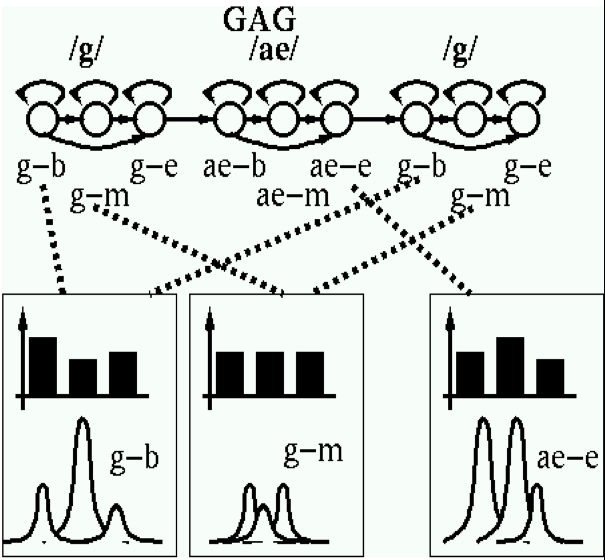
\includegraphics[width=6cm]{images/fully.png}
\caption{A fully-continuous HMM}
\label{fig:fullyContinuousHMMs}
\end{figure}

\subsubsection{Semi-continuous HMMs}
\begin{itemize}
    \item only one codebook of Gaussians in the system
    \item every acoustic model has its own set of \textit{mixture weights}
\end{itemize}
See also figure~\ref{fig:semiContinuousHMMs}.
\begin{figure}[ht]
\centering
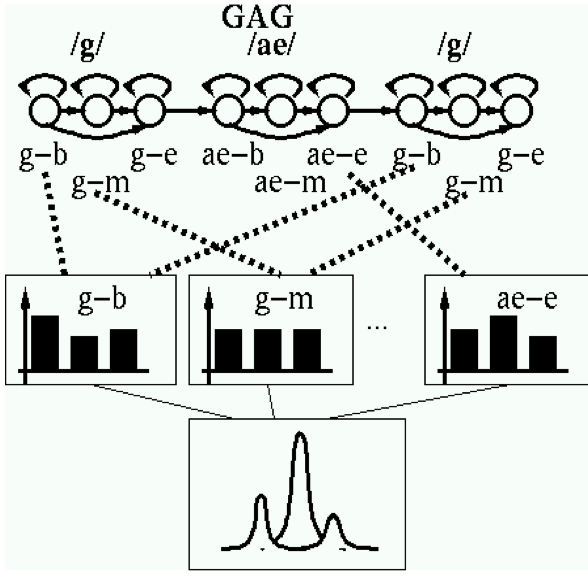
\includegraphics[width=6cm]{images/semi.png}
\caption{A semi-continuous HMM}
\label{fig:semiContinuousHMMs}
\end{figure}

\subsubsection{Phonetically-tied semi-continuous HMMs}
One codebook per phone that is shared across polyphones. For example, \textit{/g/} might have one codebook and \textit{/ae/} another.

\subsection{HMM training}

A typical HMM training session might look like this:
\begin{enumerate}
    \item Initialization:
        \begin{itemize}
            \item initialize all parameters randomly
            \item or use pre-labeled data and compute initial parameters with e.g. \textbf{k-means}
        \end{itemize}
    \item Iterative optimization / training:
        \begin{itemize}
            \item for all training utterances, run \textit{Baum-Welch} and update the HMM accordingly
            \item continue for a defined number of iterations or until there are no more improvements
        \end{itemize}
    \item Evaluation by recording an utterance and testing the HMM.
\end{enumerate}

\subsection{HMM parameter initialization}

Use labeled data:
\begin{itemize}
    \item automatic labeling
        \begin{itemize}
            \item use an existing recognizer
            \item probably suboptimal
        \end{itemize}
    \item hand-made labels
        \begin{itemize}
            \item manually assign HMM states to speech frames
            \item probably time consuming
        \end{itemize}
    \item use partial labels
\end{itemize}

